% Enable warnings about problematic code
\RequirePackage[l2tabu, orthodox]{nag}

\PassOptionsToPackage{utf8}{inputenc}
\PassOptionsToPackage{T1}{fontenc}
\PassOptionsToPackage{ngerman, american}{babel}

\documentclass{presentation}

\title[Fast Word Prediction using Top-K Joins]{\mbox{Fast and Non-Approximative} \mbox{Language Model Prefixqueries} \mbox{for Word Prediction using} \mbox{Top-k Joining Techniques}}
\subtitle{Bachelor Thesis}
\author[Lukas Schmelzeisen]{\texorpdfstring{Lukas Schmelzeisen\\\textcolor{Maroon}{\scriptsize{\texttt{\href{mailto:lukas@uni-koblenz.de}{\nolinkurl{lukas@uni-koblenz.de}}}}}}{Lukas Schmelzeisen}}
\date{August 6, 2015}
\institute[Institute for Web Science and Technologies]{Institute for Web Science and Technologies,\\University of Koblenz-Landau}

% For resizing
\usepackage{graphicx}

% For figures, equation explanation
\usepackage{standalone}
\usepackage{tikz}
\usepackage{pgfplots}
\pgfplotsset{compat = 1.12}
\usetikzlibrary{tikzmark, positioning}

% Absolute text positioning
\usepackage{textpos}

% Tables
%\usepackage{booktabs}
\usepackage{tabu}

\usepackage{appendixnumberbeamer}

\addbibresource{bibliography.bib}

\begin{document}

\begin{frame}[plain]
  \maketitle
\end{frame}

\begin{frame}[plain]
  \frametitle{Outline}

  \tableofcontents
\end{frame}


% ==============================================================================
\section{Next Word Prediction}
\subsection{}

\begin{frame}
  \frametitle{What is Next Word Prediction?}

  \begin{center}
    \LARGE Demo
  \end{center}
\end{frame}


\begin{frame}
  \frametitle{Benefits of good Word Prediction}

  \large
  \begin{itemize}
    \item Faster typing
    \item Spelling
    \item \ldots
  \end{itemize}
\end{frame}

\begin{frame}
  \frametitle{Next Word Prediction}

  \LARGE
  \begin{equation*}
    \only<1-3>{\phantom{_{p}}\NWP{\tikzmark{hist1_fst}h} = \Argmax{\mathclap{\substack{w \in \Vocab\\\phantom{p \: \text{prefix of} \: w}}}}\tikzmark{vocab_fst} \Prob{\tikzmark{w_fst}w}{\tikzmark{hist2_fst}h}}
    \only<4- >{\NWP[\tikzmark{prefix}p]{\tikzmark{hist1_snd}h} = \Argmax{\mathclap{\substack{w \in \Vocab,\\p \: \text{prefix of} \: w}}}\tikzmark{vocab_snd} \Prob{\tikzmark{w_snd}w}{\tikzmark{hist2_snd}h}}
  \end{equation*}

  \large
  
\begin{tikzpicture}[
    remember picture,
    overlay,
    expl/.style = {draw = Maroon, rounded corners, thick},
    arrow/.style = {Maroon, thick, ->, >=latex},
  ]
    \node<2->[expl]
      (hist_expl) at (2,3.5cm) {history of entered words};
    \node<3->[expl]
      (vocab_expl) at (8.5,-1.5cm) {for each word in vocabulary};
    \node<4->[expl, align=center]
      (prefix_expl) at (2.5,-1cm) {entered prefix of\\intended word};
    \LARGE % restore equation size so font relative units are correct
    \draw<2-3>[arrow] (hist_expl.south)   to [out=270, in=100] ([xshift= 0.2em, yshift= 2.0ex]{pic cs:hist1_fst});
    \draw<2-3>[arrow] (hist_expl.east)    to [out=  0, in=100] ([xshift= 0.2em, yshift= 2.0ex]{pic cs:hist2_fst});
    \draw<4- >[arrow] (hist_expl.south)   to [out=270, in=100] ([xshift= 0.2em, yshift= 2.0ex]{pic cs:hist1_snd});
    \draw<4- >[arrow] (hist_expl.east)    to [out=  0, in=100] ([xshift= 0.2em, yshift= 2.0ex]{pic cs:hist2_snd});
    \draw<3  >[arrow] (vocab_expl.north)  to [out= 90, in=  0] ([xshift=-0.7em, yshift=-1.3ex]{pic cs:vocab_fst});
    \draw<3  >[arrow] (vocab_expl.north)  to [out= 90, in=270] ([xshift= 0.4em, yshift=-0.6ex]{pic cs:w_fst});
    \draw<4- >[arrow] (vocab_expl.north)  to [out= 90, in=  0] ([xshift=-0.7em, yshift=-1.3ex]{pic cs:vocab_snd});
    \draw<4- >[arrow] (vocab_expl.north)  to [out= 90, in=270] ([xshift= 0.4em, yshift=-0.6ex]{pic cs:w_snd});
    \draw<4- >[arrow] (prefix_expl.north) to [out= 90, in=270] ([xshift= 0.2em, yshift=-0.9ex]{pic cs:prefix});
  \end{tikzpicture}
\end{frame}

\begin{frame}
  \frametitle{Goal}

  \begin{center}
    \LARGE
    Be fast!
  \end{center}
\end{frame}



% ==============================================================================
\section{Language Models}
\subsection{}

\begin{frame}
  \frametitle{How to find probabilities?}

  \begin{center}
    \LARGE $\Prob{w}{h}$ ?
  \end{center}

  \vspace{1cm}

  \onslide<2->{
    \large
    Solution: use Language Models!
  }

  \vspace{1cm}

  \onslide<3->{
    \large
    We will use two state-of-the-art Language Models:
    \begin{itemize}
      \item Modified Kneser Ney Smoothing\\[-0.4ex]{\small\parencite{ChenGoodman1309}}
      \item Generalized Language Model\\[-0.4ex]{\small\parencite{Pickhardt2014}}
    \end{itemize}
  }
\end{frame}

\begin{frame}
  \frametitle{Modified Kneser Ney Smoothing}

  \only<1-2>{
    \large
    \begin{align*}
      \ProbMKN{w_n}{w_1^{n-1}} &=
        \frac{\DiscountedCount(w_1^n) + \gamma(w_1^{n-1}) \tikzmark{recmkn_high}\ProbMKN*{w_n}{w_2^{n-1}}}
             {\Count(w_1^{n-1} \Skp)} \\
      \intertext{\vspace{0.4cm}}
      \ProbMKN*{w_n}{w_1^{n-1}} &=
        \frac{\DiscountedCount*(\WSkp w_1^n) + \gamma(w_1^{n-1}) \tikzmark{recmkn_low}\ProbMKN*{w_n}{w_2^{n-1}}}
           {\ContCountIp(\WSkp w_1^{n-1} \WSkp)}
    \end{align*}

    
\begin{tikzpicture}[
      remember picture,
      overlay,
    ]
      \draw<2>[Maroon, ultra thick] (pic cs:recmkn_high) ellipse
        [xshift=4em, yshift=0.6ex, x radius=4.5em, y radius=3ex];
      \draw<2>[Maroon, ultra thick] (pic cs:recmkn_low)  ellipse
        [xshift=4em, yshift=0.6ex, x radius=4.5em, y radius=3ex];
    \end{tikzpicture}
  }

  \only<3>{
    \begin{center}
      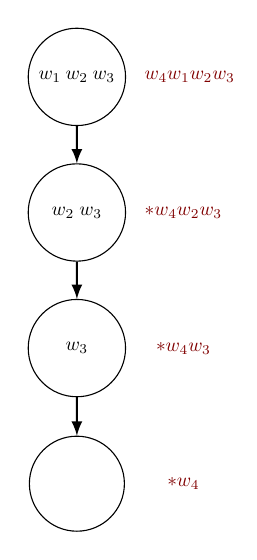
\begin{tikzpicture}
        \tikzset{
          every node/.style = {scale = 0.7},
          state/.style  = {draw, circle, align = center, text centered, text width = 4.2em},
          invis/.style  = {text width = 4.2em},
          order/.style  = {align = center, text centered, text width = 4em, text = Maroon},
        }

        \begin{scope}[node distance = 7em]
          \node [state] (highest)                    {$w_1 \: w_2 \: w_3$};
          \node [state] (lower1)  [below of=highest] {$w_2 \: w_3$};
          \node [state] (lower2)  [below of=lower1]  {$w_3$};
          \node [state] (lowest)  [below of=lower2]  {$\EmptyNGram$};
        \end{scope}

        \begin{scope}[node distance = 5.5em]
          \node [order] [right of=highest] {$\ProbMKN {w_4}{w_1 w_2 w_3}$};
          \node [order] [right of=lower1]  {$\ProbMKN*{w_4}{w_2 w_3}$};
          \node [order] [right of=lower2]  {$\ProbMKN*{w_4}{w_3}$};
          \node [order] [right of=lowest]  {$\ProbMKN*{w_4}$};
        \end{scope}

        \path[->, >=latex, thick]
          (highest) edge (lower1)
          (lower1)  edge (lower2)
          (lower2)  edge (lowest);
      \end{tikzpicture}
    \end{center}
  }
\end{frame}

\begin{frame}
  \frametitle{Generalized Language Model}

  \only<1-2>{
    \begin{align*}
      \hspace{-1.5em}
      \ProbGLM{w_n}{w_1^{n-1}} &=
        \frac{\DiscountedCount(w_1^n) + \frac{\gamma(w_1^{n-1})}{\NumSkpOp{w_1^{n-1}}}
                                        \tikzmark{recglm_high}\sum_{j=1}^{\NumSkpOp{w_1^{n-1}}} \ProbGLM*{w_n}{\SkpOp[j]{w_1^{n-1}}}}
            {\Count(w_1^{n-1} \Skp)} \\
      \intertext{\vspace{0.4cm}}
      \hspace{-1.5em}
      \ProbGLM*{w_n}{w_1^{n-1}} &=
      \frac{\DiscountedCount*(\WSkp w_1^n) + \frac{\gamma(w_1^{n-1})}{\NumSkpOp{w_1^{n-1}}}
                                              \tikzmark{recglm_low}\sum_{j=1}^{\NumSkpOp{w_1^{n-1}}} \ProbGLM*{w_n}{\SkpOp[j]{w_1^{n-1}}}}
          {\ContCountIp(\WSkp w_1^{n-1} \WSkp)}
    \end{align*}

    
\begin{tikzpicture}[
      remember picture,
      overlay,
    ]
      \draw<2>[Maroon, ultra thick] (pic cs:recglm_high) ellipse
        [xshift=6.7em, yshift=0.6ex, x radius=7.2em, y radius=4ex];
      \draw<2>[Maroon, ultra thick] (pic cs:recglm_low)  ellipse
        [xshift=6.7em, yshift=0.6ex, x radius=7.2em, y radius=4ex];
      \end{tikzpicture}
  }

  \only<3>{
    \begin{center}
      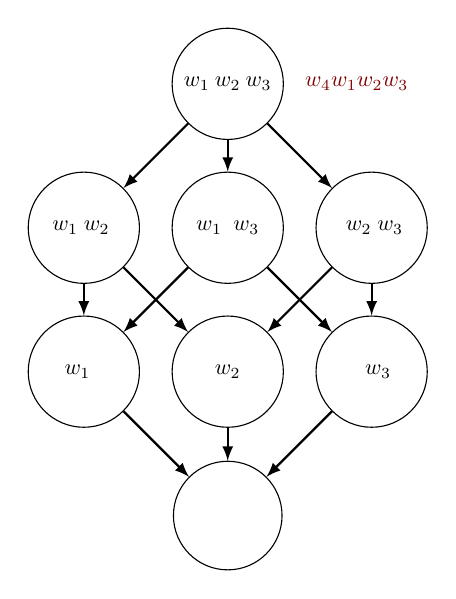
\begin{tikzpicture}
        \tikzset{
          every node/.style = {scale = 0.8},
          state/.style  = {draw, circle, align = center, text centered, text width = 4.2em},
          invis/.style  = {text width = 4.2em},
          order/.style  = {align = center, text centered, text width = 4em, text = Maroon},
        }

        \begin{scope}[node distance = 6.5em]
          \node [state] (000)                  {$w_1 \: w_2 \: w_3$};
          \node [invis] (000l) [left  of=000]  {};
          \node [invis] (000r) [right of=000]  {};

          \node [state] (001)  [below of=000l] {$w_1 \: w_2 \: \Skp$};
          \node [state] (010)  [below of=000]  {$w_1 \: \Skp \: w_3$};
          \node [state] (100)  [below of=000r] {$\Skp \: w_2 \: w_3$};

          \node [state] (011)  [below of=001] {$w_1 \: \Skp \: \Skp$};
          \node [state] (101)  [below of=010] {$\Skp \: w_2 \: \Skp$};
          \node [state] (110)  [below of=100] {$\Skp \: \Skp \: w_3$};

          \node [state] (111)  [below of=101] {$\Skp \: \Skp \: \Skp$};
          \node [invis] (111l) [below of=011] {};
          \node [invis] (111r) [below of=110] {};
        \end{scope}

        \begin{scope}[node distance = 5.5em]
          \node [order] [right of=000] {$\ProbGLM {w_4}{w_1 w_2 w_3}$};
        \end{scope}

        \path[->, >=latex, thick]
          (000) edge (001)
          (000) edge (010)
          (000) edge (100)

          (001) edge (011)
          (001) edge (101)
          (010) edge (011)
          (010) edge (110)
          (100) edge (101)
          (100) edge (110)

          (011) edge (111)
          (101) edge (111)
          (110) edge (111);
      \end{tikzpicture}
    \end{center}
  }
\end{frame}

\iffalse
\begin{frame}
  \frametitle{Backoff Graph}

  \begin{textblock}{10}(4.4,-0.9)
    \raggedleft
    \only<1>{Modified Kneser Ney Smoothing}
    \only<2>{Generalized Language Model}
  \end{textblock}

  \vspace{-0.7cm}
  \begin{center}
    \begin{tikzpicture}
      \tikzset{
        every node/.style = {scale = 0.8},
        state/.style  = {draw, circle, align = center, text centered, text width = 4.2em},
        invis/.style  = {text width = 4.2em},
        order/.style  = {align = center, text centered, text width = 4em, text = Maroon},
      }

      \only<1>{
        \begin{scope}[node distance = 7em]
          \node [state] (highest)                    {$w_1 \: w_2 \: w_3$};
          \node [state] (lower1)  [below of=highest] {$w_2 \: w_3$};
          \node [state] (lower2)  [below of=lower1]  {$w_3$};
          \node [state] (lowest)  [below of=lower2]  {$\EmptyNGram$};
        \end{scope}

        \begin{scope}[node distance = 5.5em]
          \node [order] [right of=highest] {$\ProbMKN {w_4}{w_1 w_2 w_3}$};
          \node [order] [right of=lower1]  {$\ProbMKN*{w_4}{w_2 w_3}$};
          \node [order] [right of=lower2]  {$\ProbMKN*{w_4}{w_3}$};
          \node [order] [right of=lowest]  {$\ProbMKN*{w_4}$};
        \end{scope}

        \path[->, >=latex, thick]
          (highest) edge (lower1)
          (lower1)  edge (lower2)
          (lower2)  edge (lowest);
      }

      \only<2>{
        \begin{scope}[node distance = 6.5em]
          \node [state] (000)                  {$w_1 \: w_2 \: w_3$};
          \node [invis] (000l) [left  of=000]  {};
          \node [invis] (000r) [right of=000]  {};

          \node [state] (001)  [below of=000l] {$w_1 \: w_2 \: \Skp$};
          \node [state] (010)  [below of=000]  {$w_1 \: \Skp \: w_3$};
          \node [state] (100)  [below of=000r] {$\Skp \: w_2 \: w_3$};

          \node [state] (011)  [below of=001] {$w_1 \: \Skp \: \Skp$};
          \node [state] (101)  [below of=010] {$\Skp \: w_2 \: \Skp$};
          \node [state] (110)  [below of=100] {$\Skp \: \Skp \: w_3$};

          \node [state] (111)  [below of=101] {$\Skp \: \Skp \: \Skp$};
          \node [invis] (111l) [below of=011] {};
          \node [invis] (111r) [below of=110] {};
        \end{scope}

        \path[->, >=latex, thick]
          (000) edge (001)
          (000) edge (010)
          (000) edge (100)

          (001) edge (011)
          (001) edge (101)
          (010) edge (011)
          (010) edge (110)
          (100) edge (101)
          (100) edge (110)

          (011) edge (111)
          (101) edge (111)
          (110) edge (111);
      }
    \end{tikzpicture}
  \end{center}
\end{frame}
\fi

\newcommand{\ProbMKNcab}[1]
  {\frac{\tikzmark{you_1}\DiscountedCount(\text{I love you}) + \gamma(\text{I love}) #1}{\Count(\text{I love\Skp})}}
\newcommand{\ProbMKNcb}[1]
  {\frac{\tikzmark{you_2}\DiscountedCount*(\text{\WSkp love you}) + \gamma(\text{love}) #1}{\ContCountIp(\text{\WSkp love \WSkp})}}
\newcommand{\ProbMKNc}
  {\frac{\tikzmark{you_3}\ContCountIp(\text{\WSkp you})}{\ContCountIp(\text{\WSkp \WSkp})}}

\begin{frame}
  \frametitle{Example: Probability of \enquote{you} after \enquote{I love}}

  \large
  \begin{align*}
    \hspace{-0.5cm}
    \ProbMKN {\text{you}}{\text{I love}} &= \ProbMKNcab{\ProbMKN*{\text{you}}{\text{love}}} \\
    \intertext{\vspace{0.2cm}}
    \hspace{-0.5cm}
    \ProbMKN*{\text{you}}{\text{love}}   &= \ProbMKNcb{\ProbMKN*{\text{you}}} \\
    \intertext{\vspace{0.2cm}}
    \hspace{-0.5cm}
    \ProbMKN*{\text{you}}                &= \ProbMKNc
  \end{align*}

  
\begin{tikzpicture}[
    remember picture,
    overlay,
  ]
    \draw<2->[Maroon, ultra thick] (pic cs:you_1) ellipse
      [xshift=3.2em, yshift=0.6ex, x radius=3.6em, y radius=3ex];
    \draw<2->[Maroon, ultra thick] (pic cs:you_2)  ellipse
      [xshift=3.3em, yshift=0.6ex, x radius=3.8em, y radius=3ex];
    \draw<2->[Maroon, ultra thick] (pic cs:you_3)  ellipse
      [xshift=2.6em, yshift=0.6ex, x radius=2.8em, y radius=3ex];
  \end{tikzpicture}
\end{frame}

\begin{frame}
  \frametitle{Idea: express as Weighted Sums}

  \LARGE
  \begin{equation*}
    \Prob{w}{h} = \sum_{i = 1}^{N} \tikzmark{sumweight}\SumWeight_i^h \; \tikzmark{sumarg}\SumArg_i^h(w)
  \end{equation*}

  \large
  \begin{tikzpicture}[
    remember picture,
    overlay,
    expl/.style = {draw = Maroon, rounded corners, thick},
    arrow/.style = {Maroon, thick, ->, >=latex},
  ]
    \node<2->[expl]
      (sumarg_expl) at (7.6,-1.2cm) {depends on argument $w$};
    \node<3->[expl]
      (sumweight_expl) at (6.37,3.5cm) {independent of argument $w$};
    \LARGE % restore equation size so font relative units are correct
    \draw<2->[arrow] (sumarg_expl.north)    to [out= 90, in=270] ([xshift= 1.1em, yshift=-0.9ex]{pic cs:sumarg});
    \draw<3->[arrow] (sumweight_expl.south) to [out=270, in= 90] ([xshift=-0.9em, yshift= 2.2ex]{pic cs:sumarg});
  \end{tikzpicture}
\end{frame}

\begin{frame}
  \frametitle{Evaluation of weighted sum}

  TODO
\end{frame}



% ==============================================================================
\section{Top-k Joining Techniques}
\subsection{}

\begin{frame}
  \frametitle{Completion Trie}

  \parencite{HsuOttaviano2013}
\end{frame}


\begin{frame}
  \frametitle{Threshold Algorithm}

  \begin{columns}[T]
    \begin{column}{.4\textwidth}
      \begin{enumerate}
        \item<3-> \alert< 9,13,17,19,23>{\emph{Sorted Access} to lists in any order (e.g.~round~robin)}
        \vspace{0.1cm}
        \item<4-> \alert<10,14,20>{For new words, \emph{Random Access} to to all other lists}
        \vspace{0.1cm}
        \item<5-> \alert<12,16,18,22,24>{Compute \emph{threshold} of highest possible unseen probability}
        \vspace{0.1cm}
        \item<6-> \alert<25>{Terminate when $k$ probabilities greater threshold have been found}
      \end{enumerate}
    \end{column}
    \begin{column}{.6\textwidth}
      %\vspace{-0.15cm}
      \onslide<1->{
        \begin{equation*}
          \textstyle{\Argmax{w \in \Vocab}\ProbMKN{w}{\text{I love}}}
        \end{equation*}}
      \vspace{-0.25cm}
      \onslide<2->{
        \tabulinesep=2mm
        \begin{tabu}{ l r | l r | l r }
          \tabucline[1pt]-
          \multicolumn{2}{ c }{$\EmptyNGram$} &
          \multicolumn{2}{ c }{love} &
          \multicolumn{2}{ c }{I love} \\
          \tabucline[1pt]-

          \tikzmark{tar1c1s} ~\action< 9->{the} & \action< 9->{50}~~\tikzmark{tar1c1e}&
          \tikzmark{tar1c2s}~~\action<13->{you} & \action<13->{30}~~\tikzmark{tar1c2e}&
          \tikzmark{tar1c3s}~~\action<14->{you} & \action<14->{25}~ \tikzmark{tar1c3e}\\

          \tikzmark{tar2c1s} ~\action<19->{a}   & \action<19->{40}~~\tikzmark{tar2c1e}&
          \tikzmark{tar2c2s}~~\action<10->{the} & \action<10->{20}~~\tikzmark{tar2c2e}&
          \tikzmark{tar2c3s}~~\action<20->{a}   & \action<20->{ 5}~ \tikzmark{tar2c3e}\\

          \tikzmark{tar3c1s} ~\action<14->{you} & \action<14->{35}~~\tikzmark{tar3c1e}&
          \tikzmark{tar3c2s}~~\action<20->{a}   & \action<20->{10}~~\tikzmark{tar3c2e}&
          \tikzmark{tar3c3s}~~\action<10->{the} & \action<10->{ 3}~ \tikzmark{tar3c3e}\\
        \end{tabu}}

        \vspace{-0.35cm}
        \begin{minipage}[t][3cm]{\textwidth}
          \begin{align*}
            \only< 8-11>{         \Prob[\text{threshold}] &= \infty + \infty + \infty \hspace{-0.6em} &=& \; \infty \\}
            \only<12-15>{         \Prob[\text{threshold}] &= \alert<12>{50} + \infty + \infty \hspace{-0.6em} &=& \; \infty \\}
            \only<16-17>{         \Prob[\text{threshold}] &=     50 + \alert<16>{30} + \infty \hspace{-0.6em} &=& \; \infty \\}
            \only<18-21>{         \Prob[\text{threshold}] &=     50 +     30 + \alert<18>{25} \hspace{-0.6em} &=& \;    105 \\}
            \only<22-23>{         \Prob[\text{threshold}] &=\alert<22>{40} +     30 +     25 \hspace{-0.6em} &=& \;     95 \\}
            \only<15->{\Prob{\text{you}}{\text{I love}} &= 35 + 30 + 25             \hspace{-0.6em} &=& \;  90 \\}
            \only<24-  >{         \Prob[\text{threshold}] &=     40 + \alert<24>{20} +     25 \hspace{-0.6em} &=& \;     85 \\}
            \only<11->{\Prob{\text{the}}{\text{I love}} &= 50 + 20 +  3             \hspace{-0.6em} &=& \;  73 \\}
            \only<21->{\Prob{\text{a  }}{\text{I love}} &= 40 + 10 +  5             \hspace{-0.6em} &=& \;  55 \\}
            \onslide<0>{\Prob{\text{you}}{\text{I love}} &= 50 + 30 + 25 \hspace{-0.6em} &=& \;  105}
          \end{align*}
        \end{minipage}

        
\begin{tikzpicture}[
          remember picture,
          overlay,
          iter/.style = {Maroon, thick},
        ]
          \draw< 9-18>[iter] ([yshift=-1.1ex]{pic cs:tar1c1s}) rectangle ([yshift=2.2ex]{pic cs:tar1c1e});
          \draw<13-22>[iter] ([yshift=-1.1ex]{pic cs:tar1c2s}) rectangle ([yshift=2.2ex]{pic cs:tar1c2e});
          \draw<17-  >[iter] ([yshift=-1.1ex]{pic cs:tar1c3s}) rectangle ([yshift=2.2ex]{pic cs:tar1c3e});
          \draw<19-  >[iter] ([yshift=-1.1ex]{pic cs:tar2c1s}) rectangle ([yshift=2.2ex]{pic cs:tar2c1e});
          \draw<23-  >[iter] ([yshift=-1.1ex]{pic cs:tar2c2s}) rectangle ([yshift=2.2ex]{pic cs:tar2c2e});
        \end{tikzpicture}
    \end{column}
  \end{columns}
\end{frame}

\begin{frame}
  \frametitle{No Random Access Algorithm}

  \begin{columns}[c]
     \begin{column}{.4\textwidth}
      \begin{enumerate}
        \item<2-> \emph{Sorted Access} to tries in any order
        \vspace{0.1cm}
        \item<3-> Keep track of all seen counts
        \vspace{0.1cm}
        \item<4-> Compute \emph{upper} and \emph{lower bounds} for each probability
        \vspace{0.1cm}
        \item<5-> Terminate when $k$ lower bounds greater than all other upper bounds have been found
      \end{enumerate}
     \end{column}
     \begin{column}{.6\textwidth}
     \end{column}
  \end{columns}
\end{frame}

\begin{frame}
  \frametitle{Comparison}

  TODO
\end{frame}

\begin{frame}
  \frametitle{Evaluation}

  TODO
\end{frame}


% ==============================================================================
\appendix
\begin{frame}[plain]
  \frametitle{So long, and thanks for all the fish}
\end{frame}

\section{References}
\subsection{}
\begin{frame}[allowframebreaks]
  \frametitle{References}

  \printbibliography[heading = none]
\end{frame}

\end{document}
